\begin{pages}
    \begin{Rightside}
    \selectlanguage{greek}
        \beginnumbering
		\pstart[
				\chapter{Ἡ γυνὴ Σαμαρρίας}
				\markboth{The Woman of Samaria}
				]
		\renewcommand{\LettrineFontHook}{\PHtitl}
		\lettrine[lines=3]{Ὡ}{ς} οὖν ἔγνω ὁ Κύριος ὅτι ἤκουσαν οἱ Φαρισαῖοι ὅτι Ἰησοῦς πλείονας μαθητὰς ποιεῖ καὶ βαπτίζει ἢ Ἰωάνης, —καίτοιγε Ἰησοῦς αὐτὸς οὐκ ἐβάπτιζεν ἀλλ’ οἱ μαθηταὶ αὐτοῦ, — ἀφῆκεν τὴν Ἰουδαίαν καὶ ἀπῆλθεν πάλιν εἰς τὴν Γαλιλαίαν. Ἔδει δὲ αὐτὸν διέρχεσθαι διὰ τῆς Σαμαρίας. ἔρχεται οὖν εἰς πόλιν τῆς Σαμαρίας λεγομένην Συχὰρ, πλησίον τοῦ χωρίου ὃ ἔδωκεν Ἰακὼβ Ἰωσὴφ τῷ υἱῷ αὐτοῦ· ἦν δὲ ἐκεῖ πηγὴ τοῦ Ἰακώβ. ὁ οὖν Ἰησοῦς κεκοπιακὼς ἐκ τῆς ὁδοιπορίας ἐκαθέζετο οὕτως ἐπὶ τῇ πηγῇ· ὥρα ἦν ὡς ἕκτη. 
		\pend
		\pstart
		Ἔρχεται γυνὴ ἐκ τῆς Σαμαρίας ἀντλῆσαι ὕδωρ. λέγει αὐτῇ ὁ Ἰησοῦς Δός μοι πεῖν. οἱ γὰρ μαθηταὶ αὐτοῦ ἀπεληλύθεισαν εἰς τὴν πόλιν, ἵνα τροφὰς ἀγοράσωσιν. λέγει οὖν αὐτῷ ἡ γυνὴ ἡ Σαμαρεῖτις Πῶς σὺ Ἰουδαῖος ὢν παρ’ ἐμοῦ πεῖν αἰτεῖς γυναικὸς Σαμαρείτιδος οὔσης; οὐ γὰρ συνχρῶνται Ἰουδαῖοι Σαμαρείταις. ἀπεκρίθη Ἰησοῦς καὶ εἶπεν αὐτῇ Εἰ ᾔδεις τὴν δωρεὰν τοῦ Θεοῦ, καὶ τίς ἐστιν ὁ λέγων σοι Δός μοι πεῖν, σὺ ἂν ᾔτησας αὐτὸν καὶ ἔδωκεν ἄν σοι ὕδωρ ζῶν. λέγει αὐτῷ Κύριε, οὔτε ἄντλημα ἔχεις καὶ τὸ φρέαρ ἐστὶν βαθύ· πόθεν οὖν ἔχεις τὸ ὕδωρ τὸ ζῶν; μὴ σὺ μείζων εἶ τοῦ πατρὸς ἡμῶν Ἰακώβ, ὃς ἔδωκεν ἡμῖν τὸ φρέαρ, καὶ αὐτὸς ἐξ αὐτοῦ ἔπιεν καὶ οἱ υἱοὶ αὐτοῦ καὶ τὰ θρέμματα αὐτοῦ; ἀπεκρίθη Ἰησοῦς καὶ εἶπεν αὐτῇ Πᾶς ὁ πίνων ἐκ τοῦ ὕδατος τούτου διψήσει πάλιν· ὃς δ’ ἂν πίῃ ἐκ τοῦ ὕδατος οὗ ἐγὼ δώσω αὐτῷ, οὐ μὴ διψήσει εἰς τὸν αἰῶνα, ἀλλὰ τὸ ὕδωρ ὃ δώσω αὐτῷ γενήσεται ἐν αὐτῷ πηγὴ ὕδατος ἁλλομένου εἰς ζωὴν αἰώνιον. λέγει πρὸς αὐτὸν ἡ γυνή Κύριε, δός μοι τοῦτο τὸ ὕδωρ, ἵνα μὴ διψῶ μηδὲ διέρχωμαι ἐνθάδε ἀντλεῖν. 
		\pend
		\pstart
		Λέγει αὐτῇ Ὕπαγε φώνησον τὸν ἄνδρα σου καὶ ἐλθὲ ἐνθάδε. ἀπεκρίθη ἡ γυνὴ καὶ εἶπεν Οὐκ ἔχω ἄνδρα. λέγει αὐτῇ ὁ Ἰησοῦς Καλῶς εἶπες ὅτι Ἄνδρα οὐκ ἔχω· πέντε γὰρ ἄνδρας ἔσχες, καὶ νῦν ὃν ἔχεις οὐκ ἔστιν σου ἀνήρ· τοῦτο ἀληθὲς εἴρηκας. λέγει αὐτῷ ἡ γυνή Κύριε, θεωρῶ ὅτι προφήτης εἶ σύ. οἱ πατέρες ἡμῶν ἐν τῷ ὄρει τούτῳ προσεκύνησαν· καὶ ὑμεῖς λέγετε ὅτι ἐν Ἱεροσολύμοις ἐστὶν ὁ τόπος ὅπου προσκυνεῖν δεῖ. λέγει αὐτῇ ὁ Ἰησοῦς Πίστευέ μοι, γύναι, ὅτι ἔρχεται ὥρα ὅτε οὔτε ἐν τῷ ὄρει τούτῳ οὔτε ἐν Ἱεροσολύμοις προσκυνήσετε τῷ Πατρί. ὑμεῖς προσκυνεῖτε ὃ οὐκ οἴδατε, ἡμεῖς προσκυνοῦμεν ὃ οἴδαμεν, ὅτι ἡ σωτηρία ἐκ τῶν Ἰουδαίων ἐστίν· ἀλλὰ ἔρχεται ὥρα καὶ νῦν ἐστιν, ὅτε οἱ ἀληθινοὶ προσκυνηταὶ προσκυνήσουσιν τῷ Πατρὶ ἐν πνεύματι καὶ ἀληθείᾳ· καὶ γὰρ ὁ Πατὴρ τοιούτους ζητεῖ τοὺς προσκυνοῦντας αὐτόν· Πνεῦμα ὁ Θεός, καὶ τοὺς προσκυνοῦντας ἐν πνεύματι καὶ ἀληθείᾳ δεῖ προσκυνεῖν. λέγει αὐτῷ ἡ γυνή Οἶδα ὅτι Μεσσίας ἔρχεται, ὁ λεγόμενος Χριστός· ὅταν ἔλθῃ ἐκεῖνος, ἀναγγελεῖ ἡμῖν ἅπαντα. λέγει αὐτῇ ὁ Ἰησοῦς Ἐγώ εἰμι, ὁ λαλῶν σοι. 
		\pend
		\pstart
		Καὶ ἐπὶ τούτῳ ἦλθαν οἱ μαθηταὶ αὐτοῦ, καὶ ἐθαύμαζον ὅτι μετὰ γυναικὸς ἐλάλει· οὐδεὶς μέντοι εἶπεν Τί ζητεῖς ἢ τί λαλεῖς μετ’ αὐτῆς; ἀφῆκεν οὖν τὴν ὑδρίαν αὐτῆς ἡ γυνὴ καὶ ἀπῆλθεν εἰς τὴν πόλιν, καὶ λέγει τοῖς ἀνθρώποις Δεῦτε ἴδετε ἄνθρωπον ὃς εἶπέν μοι πάντα ἃ ἐποίησα· μήτι οὗτός ἐστιν ὁ Χριστός; ἐξῆλθον ἐκ τῆς πόλεως καὶ ἤρχοντο πρὸς αὐτόν. Ἐν τῷ μεταξὺ ἠρώτων αὐτὸν οἱ μαθηταὶ λέγοντες Ῥαββεί, φάγε. ὁ δὲ εἶπεν αὐτοῖς Ἐγὼ βρῶσιν ἔχω φαγεῖν ἣν ὑμεῖς οὐκ οἴδατε. ἔλεγον οὖν οἱ μαθηταὶ πρὸς ἀλλήλους Μή τις ἤνεγκεν αὐτῷ φαγεῖν; λέγει αὐτοῖς ὁ Ἰησοῦς Ἐμὸν βρῶμά ἐστιν ἵνα ποιῶ τὸ θέλημα τοῦ πέμψαντός με καὶ τελειώσω αὐτοῦ τὸ ἔργον. οὐχ ὑμεῖς λέγετε ὅτι Ἔτι τετράμηνός ἐστιν καὶ ὁ θερισμὸς ἔρχεται; ἰδοὺ λέγω ὑμῖν, ἐπάρατε τοὺς ὀφθαλμοὺς ὑμῶν καὶ θεάσασθε τὰς χώρας, ὅτι λευκαί εἰσιν πρὸς θερισμόν. ἤδη ὁ θερίζων μισθὸν λαμβάνει καὶ συνάγει καρπὸν εἰς ζωὴν αἰώνιον, ἵνα ὁ σπείρων ὁμοῦ χαίρῃ καὶ ὁ θερίζων. ἐν γὰρ τούτῳ ὁ λόγος ἐστὶν ἀληθινὸς ὅτι ἄλλος ἐστὶν ὁ σπείρων καὶ ἄλλος ὁ θερίζων. ἐγὼ ἀπέστειλα ὑμᾶς θερίζειν ὃ οὐχ ὑμεῖς κεκοπιάκατε· ἄλλοι κεκοπιάκασιν, καὶ ὑμεῖς εἰς τὸν κόπον αὐτῶν εἰσεληλύθατε. 
		\pend
		\pstart
		Ἐκ δὲ τῆς πόλεως ἐκείνης πολλοὶ ἐπίστευσαν εἰς αὐτὸν τῶν Σαμαρειτῶν διὰ τὸν λόγον τῆς γυναικὸς μαρτυρούσης ὅτι Εἶπέν μοι πάντα ἃ ἐποίησα. ὡς οὖν ἦλθον πρὸς αὐτὸν οἱ Σαμαρεῖται, ἠρώτων αὐτὸν μεῖναι παρ’ αὐτοῖς· καὶ ἔμεινεν ἐκεῖ δύο ἡμέρας. καὶ πολλῷ πλείους ἐπίστευσαν διὰ τὸν λόγον αὐτοῦ, τῇ τε γυναικὶ ἔλεγον ὅτι Οὐκέτι διὰ τὴν σὴν λαλιὰν πιστεύομεν· αὐτοὶ γὰρ ἀκηκόαμεν, καὶ οἴδαμεν ὅτι οὗτός ἐστιν ἀληθῶς ὁ Σωτὴρ τοῦ κόσμου.
		\pend
		\pstart
		Μετὰ δὲ τὰς δύο ἡμέρας ἐξῆλθεν ἐκεῖθεν εἰς τὴν Γαλιλαίαν. αὐτὸς γὰρ Ἰησοῦς ἐμαρτύρησεν ὅτι προφήτης ἐν τῇ ἰδίᾳ πατρίδι τιμὴν οὐκ ἔχει. ὅτε οὖν ἦλθεν εἰς τὴν Γαλιλαίαν, ἐδέξαντο αὐτὸν οἱ Γαλιλαῖοι, πάντα ἑωρακότες ὅσα ἐποίησεν ἐν Ἱεροσολύμοις ἐν τῇ ἑορτῇ· καὶ αὐτοὶ γὰρ ἦλθον εἰς τὴν ἑορτήν. 
		\pend
		\pstart
		Ἦλθεν οὖν πάλιν εἰς τὴν Κανὰ τῆς Γαλιλαίας, ὅπου ἐποίησεν τὸ ὕδωρ οἶνον. Καὶ ἦν τις βασιλικὸς οὗ ὁ υἱὸς ἠσθένει ἐν Καφαρναούμ· οὗτος ἀκούσας ὅτι Ἰησοῦς ἥκει ἐκ τῆς Ἰουδαίας εἰς τὴν Γαλιλαίαν, ἀπῆλθεν πρὸς αὐτὸν καὶ ἠρώτα ἵνα καταβῇ καὶ ἰάσηται αὐτοῦ τὸν υἱόν· ἤμελλεν γὰρ ἀποθνήσκειν. εἶπεν οὖν ὁ Ἰησοῦς πρὸς αὐτόν Ἐὰν μὴ σημεῖα καὶ τέρατα ἴδητε, οὐ μὴ πιστεύσητε. λέγει πρὸς αὐτὸν ὁ βασιλικός Κύριε, κατάβηθι πρὶν ἀποθανεῖν τὸ παιδίον μου. λέγει αὐτῷ ὁ Ἰησοῦς Πορεύου· ὁ υἱός σου ζῇ. ἐπίστευσεν ὁ ἄνθρωπος τῷ λόγῳ ὃν εἶπεν αὐτῷ ὁ Ἰησοῦς, καὶ ἐπορεύετο. ἤδη δὲ αὐτοῦ καταβαίνοντος οἱ δοῦλοι ὑπήντησαν αὐτῷ λέγοντες ὅτι ὁ παῖς αὐτοῦ ζῇ. ἐπύθετο οὖν τὴν ὥραν παρ’ αὐτῶν ἐν ᾗ κομψότερον ἔσχεν· εἶπαν οὖν αὐτῷ ὅτι Ἐχθὲς ὥραν ἑβδόμην ἀφῆκεν αὐτὸν ὁ πυρετός. ἔγνω οὖν ὁ πατὴρ ὅτι ἐκείνῃ τῇ ὥρᾳ ἐν ᾗ εἶπεν αὐτῷ ὁ Ἰησοῦς Ὁ υἱός σου ζῇ· καὶ ἐπίστευσεν αὐτὸς καὶ ἡ οἰκία αὐτοῦ ὅλη. Τοῦτο δὲ πάλιν δεύτερον σημεῖον ἐποίησεν ὁ Ἰησοῦς ἐλθὼν ἐκ τῆς Ἰουδαίας εἰς τὴν Γαλιλαίαν.
		\pend
        \endnumbering
    \end{Rightside}
    \begin{Leftside}
        \beginnumbering
        \pstart[
        			\chapter{The Woman of Samaria}
        	   ]
        \renewcommand\LettrineFontHook{\Zallmanfamily}
		\lettrine[lines=3]{W}{hen} the Lord, therefore, knew that the Pharisees had heard that Jesus was making and baptising more disciples than John — even tough Jesus did not baptise (them) himself —, he left Judea and left for Galilee. (In order to get there), he had to walk through Samaria. He went, then, to a city of Samaria called Sychar (which was) close to the region which Jacob gave to Joseph, his son; (and) there was a well of Jacob’s there (or Jacob’s Well). Jesus, therefore, having grown weary (tired) because of his journey, sat down upon the well (when the) time was approximately six (roughly noon). 
		\pend
		\pstart		
		There (then) came a woman of Samaria (to the well) to draw (some) water (from it) and Jesus tells her, “Give me something to drink.” (He had to ask her) because his disciples left to go into the city to buy some food. The Samaritan woman then says to him, “How can you — being a Jew — ask for something to drink from me, a Samaritan woman? For (you know that) the Jews do not have dealings with the Samaritans.” Jesus answered and told her, “If you knew the gift of God and (if you knew) who was telling you: ‘give me something to drink’ — (if you really knew this) then you would have asked him (to give water to you) and he would have given you living water.” And the woman tells him, “(But) sir, you have nothing to draw water with and the well is deep; from where do you have living water (where did you get that living water of yours from)? Surely you are not greater than our father Jacob, who gave us this well and from which he himself — and his children and his livestock — have drunk?” Jesus answered and said to her, “Everyone who drinks from this water will be thirsty again (at some point); (but) whoever drinks from the water which I shall give them will not be thirsty again for eternity — instead, the water I shall give them will turn into a well within them, springing up into eternal life.” The woman says to him, “Sir, give me this water, so that I will never be thirsty again (and so that I will never have to) come here again to draw water.” 
		\pend
		\pstart
		He, then, says to her, “Get up, call your husband and come here (again).” The woman answered him and said, “I do not have a husband (man).” And Jesus tells her, “You said well that you have no husband (man). For you have had five husbands (men) (already), and he whom you now have is not (truly) your husband (man). This you said truthfully.” The woman tells him, “Sir, I (can) see that you are a prophet. Our fathers worshipped God in this mountain (Mount Gerizim), but you say that that the place to worship God is in Jerusalem.” Jesus tells her, “Believe me, woman, that the hour shall come in which you shall worship the Father neither in Jerusalem nor in this mountain. You worship that which you do not know, (but) we worship that which we know — for the salvation is from the Jews (i. e. The Messiah will be a Jew and not a Gentile or Samaritan). But the hour will come — and has already come — when the true worshippers will worship the Father in spirit and in truth; because the Father seeks such people to worship him. God is a spirit, and his worshippers must worship him in spirit and in truth.” And the woman tells him, “I know that the Messiah will come (which means ‘The Anointed One’); and when comes, he will tells us everything.” And Jesus tells her, “The one you are speaking of is I.”
		\pend
		\pstart
		At this moment, his disciples arrived and they were amazed that he was speaking to a (the?) woman. But none of them asked (things such as): “What do you want?” or “Why are you speaking to her?” Leaving her water jar, she left for the city and told the people (there), “Come and see the man who told me all the things I have ever done. Is this not the Anointed One?” They left the city and went to him. In the meantime, his disciples were asking him saying, “Teacher, (please) eat.” He told them, “I have food to eat which you do not know of.” The disciples were saying to one another, “Has nobody brought him any food?” And Jesus says to them, “My food is doing the will of him who sent me and to finish his work. Did you not (once) say, ‘Only four months until harvest comes?’ Look, I tell you: lift up your eyes and see that the fields are already white for harvest. They who harvest will receive wages and gather fruit unto eternal life, so that the sower may rejoice together with the reaper. For in this the saying is true: ‘One sows and another reaps.’ I have sent you to reap that which you did not work for; others have laboured and you have been entered into their labour.”
		\pend
		\pstart
		Many of the Samaritans from that city believed in him because of the woman’s testimony: “He told me all the things I have ever done”. When the Samaritans had walked to him, they asked him to stay with them — and he stayed there for two days. And many more believed (in him) because of his own words; and to the woman they said, “We no longer believe (in him) because of what you said; for we have heard ourselves, and we know (now) that he truly is the Saviour of the cosmos (world).”
		\pend
		\pstart
		After the two days (had passed), he departed and left for Galilee. For Jesus himself testified that a prophet does not have any honour in his own homeland. As he arrived in Galilee, the Galileans welcomed him because they had seen all the things he had done at the feast; for they had gone to the feast themselves. 
		\pend
		\pstart
		Thus, he, once again, went to Cana of Galilee — (the place) where he had turned water to wine. And there was a royal official there, whose son was lying sick in Capernaum. He — having heard of Jesus’ coming from Judea to Galilee — went to Jesus and asked (him) if he could come down (to Capernaum) and heal his son — for he was about to die. Jesus, therefore, told him, “You do not believe unless you see signs and wonders?” And the royal official tells him, “Sir, (please) come down (to Capernaum) before my son’s death.” And Jesus tells him, “Go. Your son lives.” The man believed the words which Jesus had spoken to him and left. As he had gone down (and arrived), his servants met him and told him, “Your son lives.” He, then, inquired of them at which time he had gotten better; and they said, “His fever left him yesterday at seven (1 pm).” The father knew that it was during that hour in which Jesus told him, “Your son lives.” And he — and his entire family (household) — believed. This second sign Jesus did after coming from Judea and going into Galilee.
		\pend
        \endnumbering
    \end{Leftside}
\end{pages} 
\Pages

\clearpage
\thispagestyle{empty}
\null\vfill
\settowidth\longest{\huge\itshape […] and when I turned around I saw}
\begin{center}
\parbox{\longest}{%
  \raggedright{\huge\itshape%
    ``Give me something to drink.'' \par\bigskip
  }
  \raggedleft\Large\MakeUppercase{Christ and the Woman of Samaria — 1655, Rembrandt}\par%
}
\vfill\vfill
\clearpage\newpage
\end{center}
\newpage
\thispagestyle{empty}
\begin{center}
	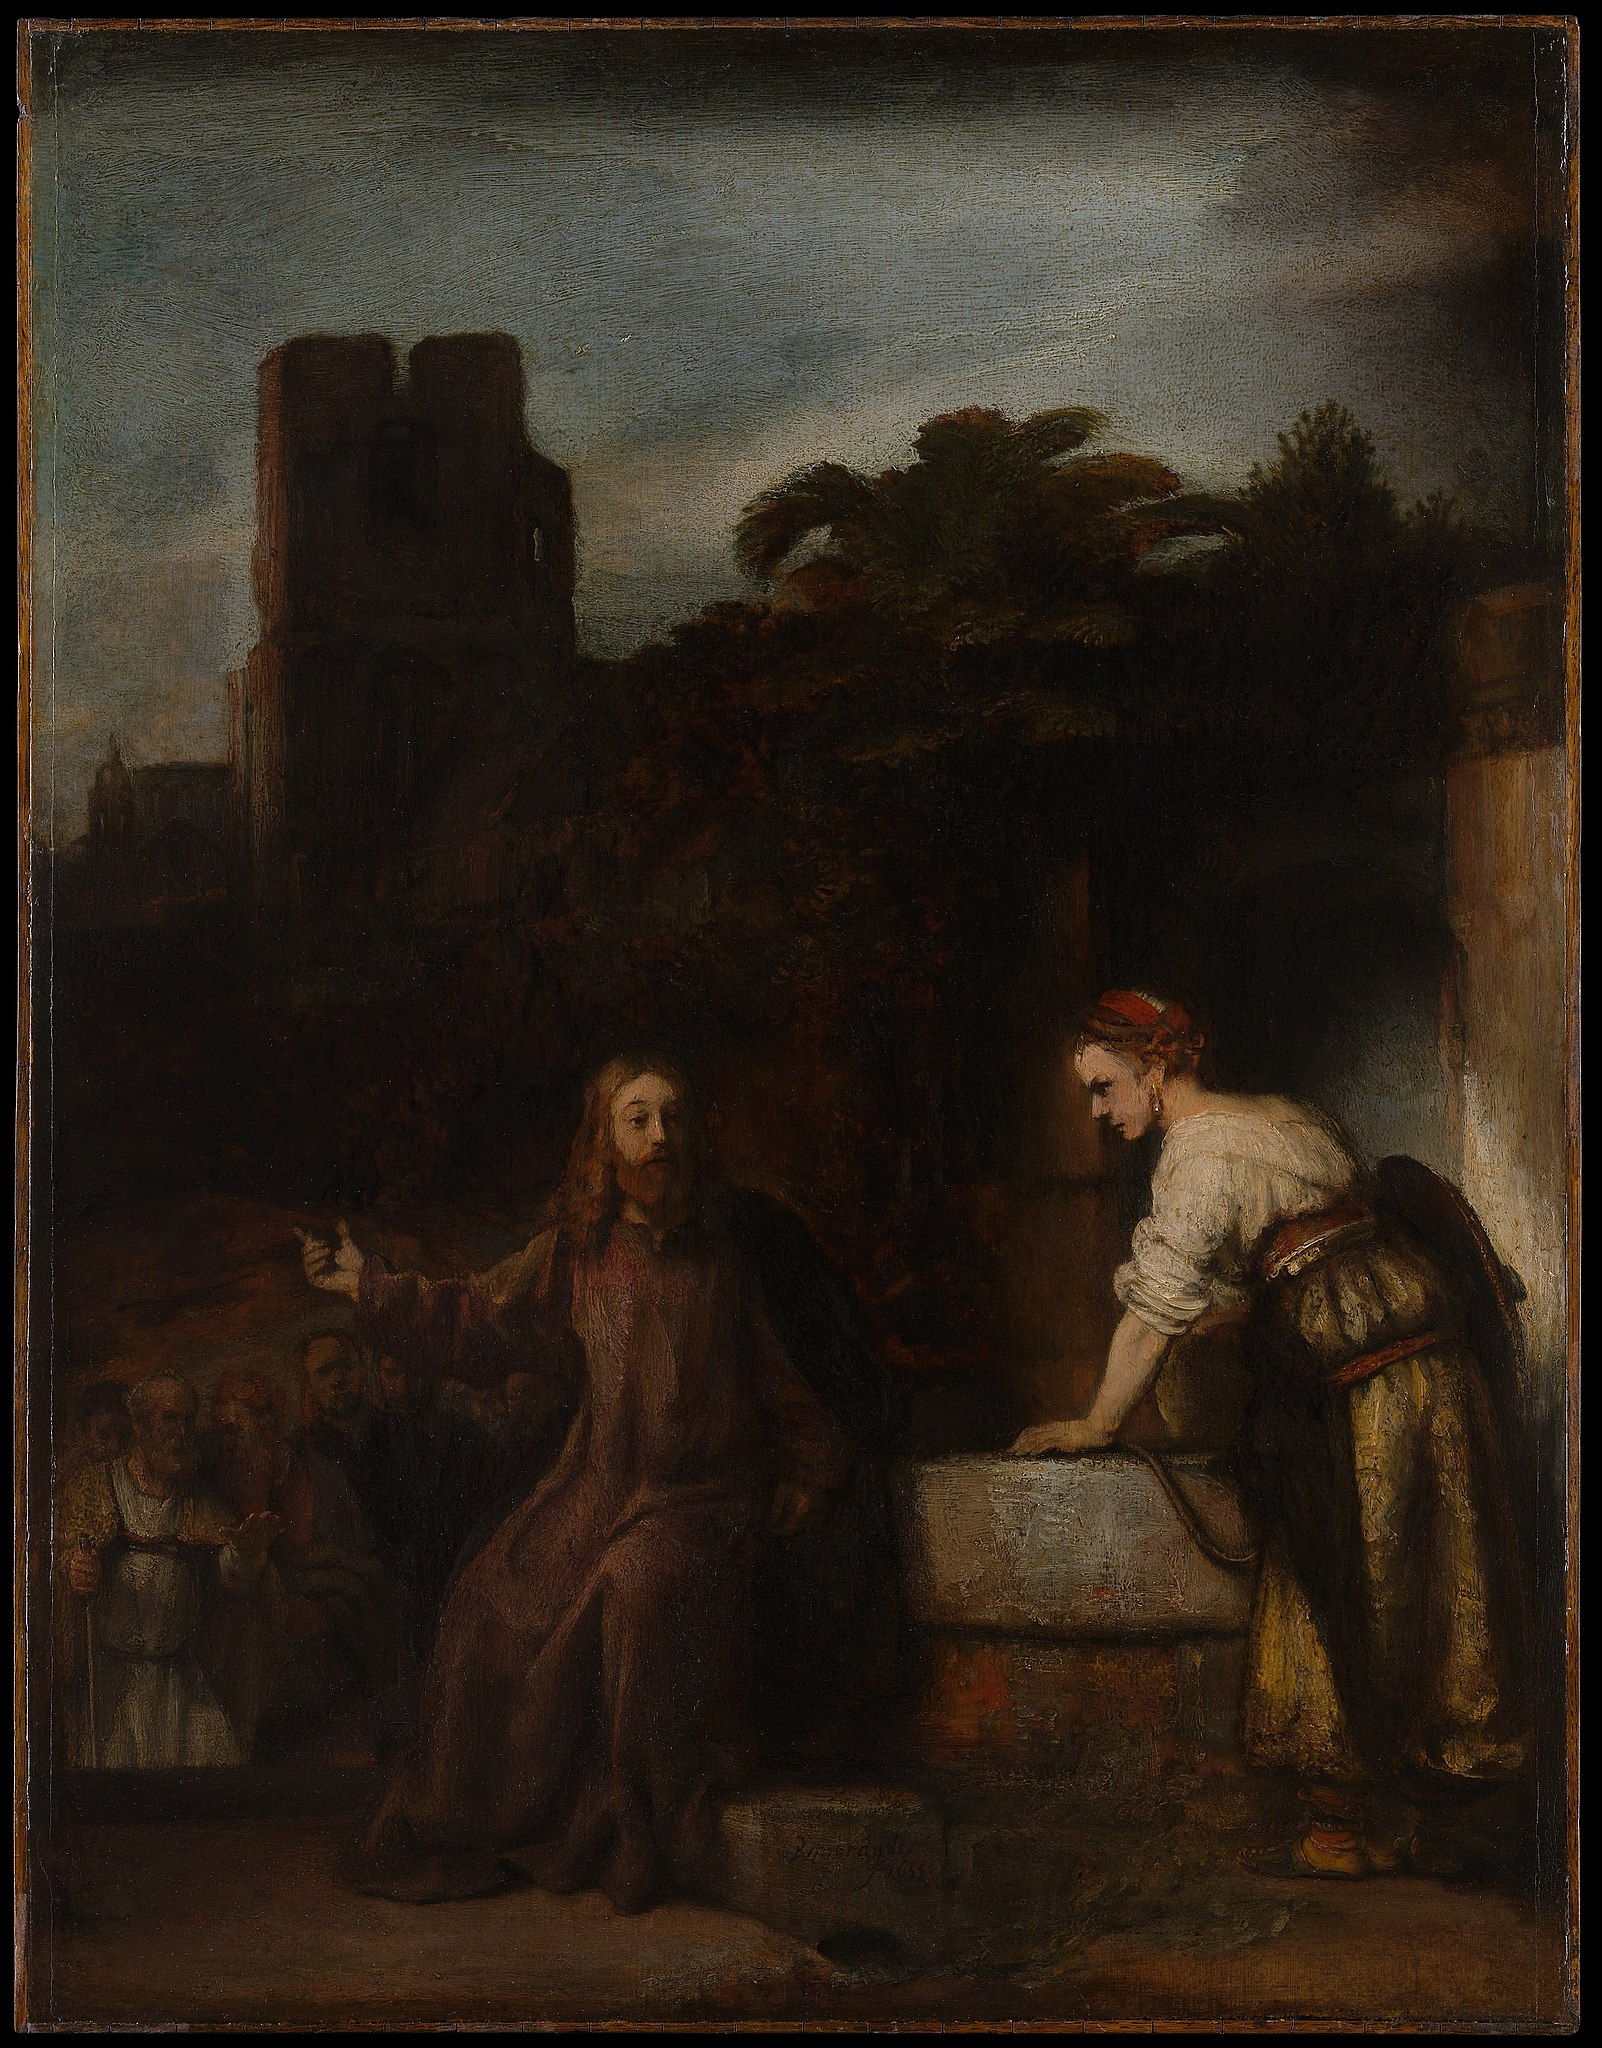
\includegraphics[width=1\textwidth]{images/illustrations/jesuswomansamaria.jpeg}
\end{center}
\vfill\vfill